\subsection{Finite Volume Method}
\label{subsec:finite_volume_method}

The Finite Volume Method (FVM) is a numerical technique used to discretize partial differential equations, and is particularly well suited for the discretization of the Navier-Stokes equations.

The idea here is to divide the domain into a set of control volumes, and then integrate the governing equations over each control volume.
The resulting set of equations will be a set of algebraic equations, which can be solved using a discrete calculator.


\subsubsection{Control volumes}

Before proceeding with the discretization of the governing equations, we need to define what a control volume is and the notations used in the rest of the document.

In particular, we will assume from now on to have a Cartesian grid, with a uniform mesh spacing in both the $x$ and $y$ directions.

From the Figure \ref{fig:control_volume}, we can appreciate graphically how the domain is divided.

\begin{figure}[H]
    \centering
    \def\nCV{5}
    \def\dX{1.5cm}
    \def\dY{1.5cm}
    \def\labelsH{{"WW", "W", "P", "E", "EE"}}
    \def\labelsV{{"SS", "S", "P", "N", "NN"}}

    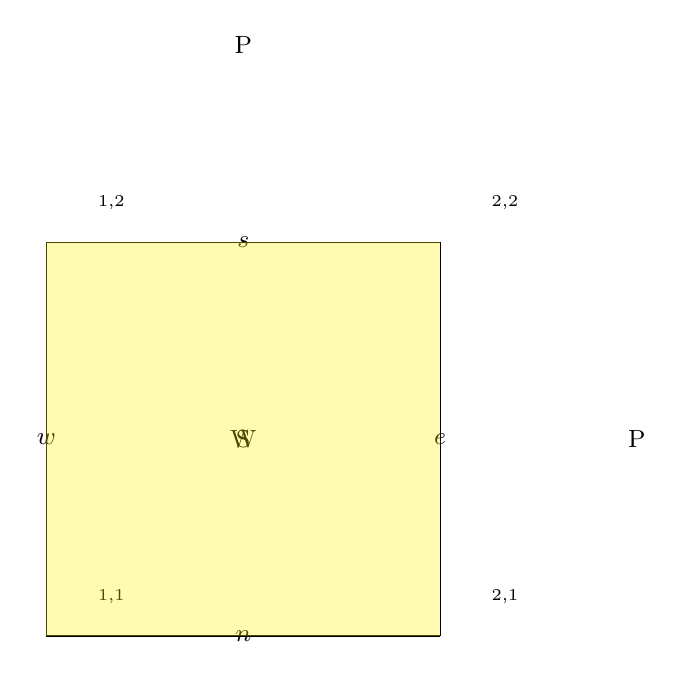
\begin{tikzpicture}

        \foreach \n in {0,1,...,\nCV}
            {
                \draw (0, \n*\dY) -- (\nCV*\dX, \n*\dY);
                \draw (\n*\dX, 0) -- (\n*\dX, \nCV*\dY);
            }

        % \foreach \n in {0,1,...,\the\numexpr\nCV-1\relax}
        %     {
        %         \draw[dashed] (-\dX/2, \n*\dY + \dY/2) -- (\nCV*\dX+\dX/2, \n*\dY + \dY/2);
        %         \draw[dashed] (\n*\dX + \dX/2, -\dY/2) -- (\n*\dX + \dX/2, \nCV*\dY+\dY/2);
        %     }

        \foreach \y in {0,1,...,\the\numexpr\nCV-1\relax}
            {
                \foreach \x in {0,1,...,\the\numexpr\nCV-1\relax}
                    {
                        \node[font=\small] at (\x*\dX+\dX/6, \y*\dY+\dY/10) {$_{\the\numexpr\x+1\relax,\the\numexpr\y+1\relax}$};
                    }
            }

        \foreach \n in {0,1,...,\the\numexpr\nCV-1\relax}
            {
                \node[font=\small] at (\n*\dX+\dX/2, \nCV/2*\dY) {\pgfmathparse{\labelsH[\n]}\pgfmathresult};
                \node[font=\small] at (\nCV/2*\dX, \n*\dY+\dY/2) {\pgfmathparse{\labelsV[\n]}\pgfmathresult};
            }

        \node[font=\small] at (\nCV/2*\dX, \nCV/2*\dY+\dY/2) {$s$};
        \node[font=\small] at (\nCV/2*\dX, \nCV/2*\dY-\dY/2) {$n$};
        \node[font=\small] at (\nCV/2*\dX-\dX/2, \nCV/2*\dY) {$w$};
        \node[font=\small] at (\nCV/2*\dX+\dX/2, \nCV/2*\dY) {$e$};

        \fill[yellow, opacity=0.3] (\nCV/2*\dX-\dX/2, \nCV/2*\dY-\dY/2) rectangle (\nCV/2*\dX+\dX/2, \nCV/2*\dY+\dY/2);

    \end{tikzpicture}
    \caption{Control volumes and control volume faces.}
    \label{fig:control_volume}
\end{figure}

In particular, Figure \ref{fig:control_volume} shows:

\begin{itemize}
    \item A grid of control volumes, with the subscript $(i,j)$ indicating the position of the control volume in the $x$ and $y$ directions, respectively. For example, the control volume in the center of the grid has indices $(i,j)=(3,3)$.
    \item The control volume centers with capital letters, $P, N, S, E, W, \ldots$.
    \item The control volume faces with lowercase letters, $n, s, e, w$.
\end{itemize}

Notice also that the capital letters always refers to a relative position with respect to the control volume in consideration.
For example, $P$ refers to the control volume in consideration, $N$ refers to the control volume to the north of $P$, and so on.
For this reason, in Figure \ref{fig:control_volume}, the control volume $P$ is highlighted in yellow so to indicate that is the control volume in consideration.


\subsubsection{Staggered grid and $L_{shape}$}

As we will see later during the formulation of the solving solution, for the purpose of this work, we will use a specific type of grid, called staggered grid.

We can also give a brief definition of the two types of grids available in the literature, which are:

\begin{itemize}
    \item \textbf{Collocated grid}: all the variables are located at the same point in the control volume (e.g. the center of the control volume).
    \item \textbf{Staggered grid}: the variables are located at different points in the control volume (e.g. the velocity components are located at the center of the faces of the control volume, and the pressure is located at the center of the control volume).
\end{itemize}

Given the formulation of the staggered grid, it's now useful to define the so called $L_{shape}$, which is a frame used to define in a compact and clear way the position of the variables in the control volume.

The $L_{shape}$ has been reported for control volume $P$ in Figure \ref{fig:L_shape}.

\begin{figure}[H]
    \centering
    \def\nCV{3}
    \def\dX{3cm}
    \def\dY{3cm}
    \def\labelsH{{"W", "P", "E"}}
    \def\labelsV{{"S", "P", "N"}}

    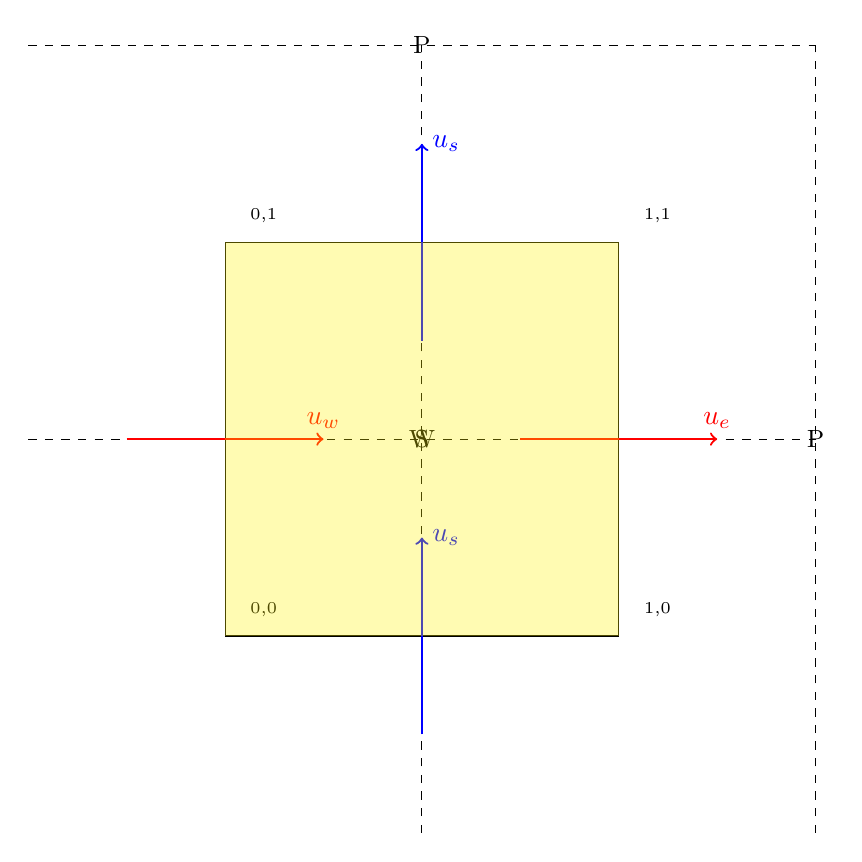
\begin{tikzpicture}

        \foreach \n in {0,1,...,\nCV}
            {
                \draw (0, \n*\dY) -- (\nCV*\dX, \n*\dY);
                \draw (\n*\dX, 0) -- (\n*\dX, \nCV*\dY);
            }

        \foreach \n in {0,1,...,\the\numexpr\nCV-1\relax}
            {
                \draw[dashed] (-\dX/2, \n*\dY + \dY/2) -- (\nCV*\dX+\dX/2, \n*\dY + \dY/2);
                \draw[dashed] (\n*\dX + \dX/2, -\dY/2) -- (\n*\dX + \dX/2, \nCV*\dY+\dY/2);
            }

        \foreach \y in {0,1,...,\the\numexpr\nCV-1\relax}
            {
                \foreach \x in {0,1,...,\the\numexpr\nCV-1\relax}
                    {
                        \node[font=\small] at (\x*\dX+\dX/10, \y*\dY+\dY/15) {$_{\the\numexpr\x-(\nCV-1)/2\relax,\the\numexpr\y-(\nCV-1)/2\relax}$};
                    }
            }

        \foreach \n in {0,1,...,\the\numexpr\nCV-1\relax}
            {
                \node[font=\small] at (\n*\dX+\dX/2, \nCV/2*\dY) {\pgfmathparse{\labelsH[\n]}\pgfmathresult};
                \node[font=\small] at (\nCV/2*\dX, \n*\dY+\dY/2) {\pgfmathparse{\labelsV[\n]}\pgfmathresult};
            }

        \draw[thick, blue, ->] (\nCV/2*\dX, \nCV/2*\dY)++(0,  \dY/4) -- ++(0, \dY/2) node[pos=1, right] {$u_s$};
        \draw[thick, blue, ->] (\nCV/2*\dX, \nCV/2*\dY)++(0, -\dY/2-\dY/4) -- ++(0, \dY/2) node[pos=1, right] {$u_s$};
        \draw[thick, red, ->] (\nCV/2*\dX, \nCV/2*\dY)++(\dX/4, 0) -- ++(\dX/2, 0) node[pos=1, above] {$u_e$};
        \draw[thick, red, ->] (\nCV/2*\dX, \nCV/2*\dY)++(-\dX/2-\dX/4, 0) -- ++(\dX/2, 0) node[pos=1, above] {$u_w$};

        \fill[yellow, opacity=0.3] (\nCV/2*\dX-\dX/2, \nCV/2*\dY-\dY/2) rectangle (\nCV/2*\dX+\dX/2, \nCV/2*\dY+\dY/2);

    \end{tikzpicture}
    \caption{$L_{shape}$ for control volume $P$.}
    \label{fig:L_shape}
\end{figure}

Basically, the $L_{shape}$ for control volume $P$ links the velocity components to the control volume $P$ itself, and it's used to define the indexes of the system.

In particular, the same Figure \ref{fig:L_shape} can be represented using the index notations, as shown in Figure \ref{fig:L_shape_index}.

\begin{figure}[H]
    \centering
    \def\nCV{1}
    \def\dX{5cm}
    \def\dY{5cm}

    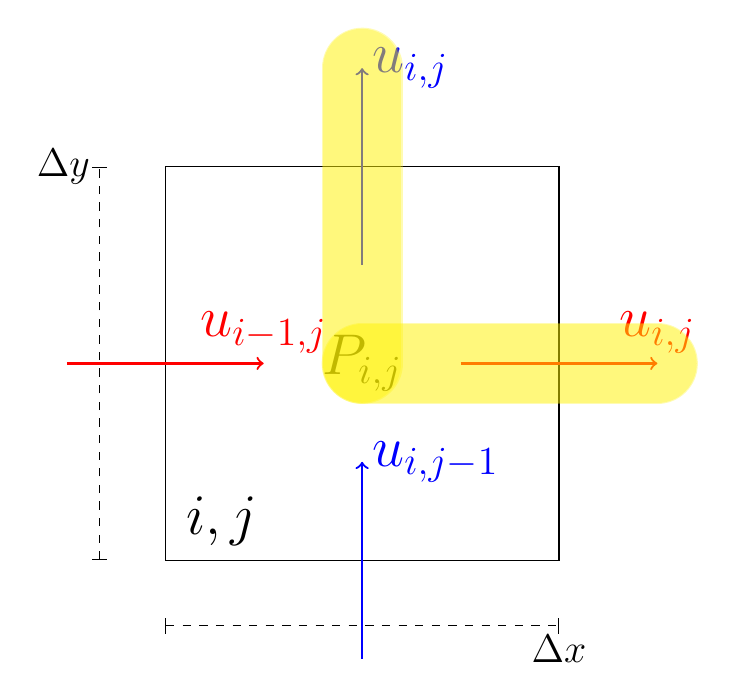
\begin{tikzpicture}[every node/.style={font=\huge}]

        \draw (0, 0) -- (\dX, 0) -- (\dX, \dY) -- (0, \dY) -- cycle;

        \node at (\dX/7, \dY/10) {$i,j$};

        \node at (\dX/2, \dY/2) {$P_{i,j}$};

        \draw[thick, blue, ->] (\dX/2, \dY/2)++(0,  \dY/4) -- ++(0, \dY/2) node[pos=1, right] {$u_{i,j}$};
        \draw[thick, blue, ->] (\dX/2, \dY/2)++(0, -\dY/2-\dY/4) -- ++(0, \dY/2) node[pos=1, right] {$u_{i,j-1}$};
        \draw[thick, red, ->] (\dX/2, \dY/2)++(\dX/4, 0) -- ++(\dX/2, 0) node[pos=1, above] {$u_{i,j}$};
        \draw[thick, red, ->] (\dX/2, \dY/2)++(-\dX/2-\dX/4, 0) -- ++(\dX/2, 0) node[pos=1, above] {$u_{i-1,j}$};

        \draw[yellow,
            opacity=0.3,
            line cap=round,
            double=yellow,
            double distance=\dX/5,
        ] (\dX/2, \dY/2) -- ++(0, \dY/2+\dY/4);

        \draw[yellow,
            opacity=0.3,
            line cap=round,
            double=yellow,
            double distance=\dX/5,
        ] (\dX/2, \dY/2) -- ++(\dX/2+\dX/4, 0);

        \draw[dashed, |-|] (0, -\dY/6) -- (\dX, -\dY/6) node[pos=1, below, font=\Large] {$\Delta x$};
        \draw[dashed, |-|] (-\dX/6, 0) -- (-\dX/6, \dY) node[pos=1, left, font=\Large] {$\Delta y$};

    \end{tikzpicture}
    \caption{$L_{shape}$ for control volume $P$ using index notations.}
    \label{fig:L_shape_index}
\end{figure}

From Figure \ref{fig:L_shape_index}, we can appreciate how the $L_{shape}$ works well with index notations, and can be useful when working purely with indexes to refer to the variables.